\documentclass[twoside,spanish,a4paper,12pt]{tfg}
\usepackage[table,xcdraw]{xcolor}
\usepackage{array}
\usepackage{longtable}
\usepackage{multirow}
\usepackage{float}
\usepackage{tikz}
\usetikzlibrary{arrows.meta, shapes.geometric, positioning}


% Editar la titulación
\titulacion{Grado en Ingeniería \\ Multimedia}

% Editar el título
\title{Diseño e implementación de un teclado virtual multilingüe para proyectos de VR}

% Si es una alumna se debe usar
% \authorlabel{Autora}
\authorlabel{Autor}
% Editar el nombre
\author{Jonathan David Signes Falcó}


% Si hay varios tutores:
% \tutorlabel{Tutores}
% \tutor{Nombre del tutor 1 \\[2mm] Nombre del turor2}
% Si el tutor es masculino:
% \tutorlabel{Tutor}
\tutorlabel{Tutor}
% Editar
\tutor{Javier Peris Sevilla}

% Editar: Poner mes y año de la convocatoria de lectura del TFM
\convocatoria{Marzo 2025}

\begin{document}
	
	% NO QUITAR ESTOS ELEMENTOS
	\portada
	\cleardoublepage
	\contraportada
	\cleardoublepage
	\declaracion
	\cleardoublepage
	
	
	% Editar: Resumen en Español (obligatorio)
	\begin{resumen}
		Diseño e implementación de un teclado virtual configurable para tener una simulación de un teclado físico y un teclado plano .
		
		Este estaría hecho con Unity y estarían implementados siete u ocho idiomas cuyos teclados usen sus propios caracteres. Entre estos estarían el ruso, alemán, francés, español, griego coreano y árabe.
	\end{resumen}
	\cleardoublepage
	
	% Editar: Resumen en Inglés
	\begin{abstract}
		Disseny i implementació d'un teclat virtual configurable per a tindre una simulació d'un teclat físic i un teclat pla.
		
		Aquest estaria fet amb Unity i estarien implementats set o huit idiomes els teclats dels quals usen els seus propis caràcters. Entre ells estarien el rus, alemany, francés, espanyol, grec, coreà i àrab.
	\end{abstract}
	\cleardoublepage
	
	% Editar: Resumen en Valenciano
	\begin{resum}
		Design and implementation of a configurable virtual keyboard to simulate a physical keyboard and a flat keyboard.
		
		This would be made with Unity and would implement seven or eight languages whose keyboards use their own characters. These would include Russian, German, French, Spanish, Greek, Korean, and Arabic.
	\end{resum}
	\cleardoublepage
	
	
	% Editar: Agradecimientos (opcional)
	\begin{agradecimientos}
		En primer lugar quiero agradecer a todos aquellos que me han apoyado durante estos años, en especial al profesorado que me ha acompañado en las distintas etapas de mi vida académica, han sabido ver en mi valores y capacidades que han ido desarrollándose.
		
		Asimismo quiero dar las gracias a mi familia por apoyarme incondicionalmente y soportar mis desvelos con cariño y paciencia.
	\end{agradecimientos}
	\cleardoublepage
	
	\tableofcontents
	
	\pagestyle{tfg}
	\justify
	
	% Las figuras se buscan en el directorio figs
	
	% Cada capítulo está en su propio fichero tex. Ver el directorio tex.
	
	% La bibliografía está dentro del directorio bib
	\chapter{Introducción}
	% Contenidos del capítulo.
% Las secciones presentadas son orientativas y no representan
% necesariamente la organización que debe tener este capítulo.

\section{Introducción}


\section{Motivación}


\section{Objetivos}


\section{Organización de la memoria}

	
	\chapter{Estado del arte}
	% Contenidos del capítulo.
% Las secciones presentadas son orientativas y no representan
% necesariamente la organización que debe tener este capítulo.

\section{Análisis de aplicaciones similares}
% Qué aplicaciones similares hay y en qué se diferencia de ellas la propuesta
Como el TFG no se trata de una aplicación per se, si no de un asset destinado a el Asset Store de Unity, se puede determinar que no hay aplicaciones similares en el mercado tecnológico. No obstante, sí se pueden encontrar veintinueve Assets de teclados para realidad virtual en total, que oscilan entre la gratuidad y precios de hasta 359.27€. 

Los teclados de gama baja parecen muy simples respecto a uso, funciones y customización. Los de gama media son muy personalizables. En cuanto a la gama alta de teclados, destaca su robustez y capacidad para usos múltiples en todo el sistema. 

Para distinguirme de todos estos, decidí diseñar un teclado con el que se pueda escribir en varios idiomas, ya que ninguno de los veintinueve teclados antes mencionados poseen esta característica, acortando su rango de mercado, puesto que se limitan a la lengua inglesa.

\section{Tecnologías}
% Análisis crítico de las tecnologías y sistemas de despliegue posibles y por qué se han seleccionado unas concretas.
Para el desarrollo del teclado multilingüe en realidad virtual, se han considerado diversas tecnologías y sistemas de despliegue. A continuación, se presentan las opciones analizadas y las razones detrás de la selección final.

\textbf{Tecnologías de Desarrollo}

\textbf{-Unity:} Unity se seleccionó como la plataforma principal de desarrollo debido a su flexibilidad y robusto soporte para aplicaciones de RV. Su capacidad para integrarse con pluguins como TextMeshPro y mi entendimiento de esta por el grado estudiado fueron factores determinantes. Además permite el desarrollo en diversas plataformas, con lo que se alcanza una mayor audiencia, sumandose al factor de los múltiples idiomas.

\textbf{-Unreal Engine:} Aunque Unreal Engine ofrece gráficos de alta calidad y herramientas avanzadas para el desarrollo de RV, su curva de aprendizaje es más pronunciada y dado a que debería de haber aprendido de cero, el tiempo requerido para la realización del proyecto se habría prolongado excesivamente, volviéndose inviable para terminar en el plazo requerido. Dado el enfoque del proyecto en la usabilidad y la eficiencia del desarrollo, Unity fue la opción preferida. Además, la gestión de recursos y la documentación extensa en Unity facilitaron la implementación del teclado multilingüe.

\textbf{Sistemas de despliegue}

\textbf{-Asset Store:} Asset store se seleccionó como uno de los sistemas de despliegue por distintos motivos. Es una plataforma muy conocida y ampliamente utilizada por los desarrolladores, lo que brinda una altísima exposición. El hecho de que el asset esté disponible en el Asset Store de Unity puede servir como una validación de su calidad y utilidad. Los usuarios pueden confiar en que los assets han pasado por un proceso de revisión y cumplen con los estándares de calidad de Unity, lo que puede aumentar la credibilidad y la confianza en el producto. Es muy fácil descubrir, adquirir y administrar los distintos assets ya que utiliza la infraestructura existente de Unity para la distribución y gestión de estos. La publicación aquí te permite actualizar regularmente los assets y ofrecer soporte a los usuarios de manera eficiente. Los usuarios pueden recibir notificaciones automáticas de actualizaciones y acceder fácilmente a la documentación y el soporte técnico que proporciones a través de la plataforma. Y por último, pero no menos importante, ofrece la posibilidad de monetizar tu trabajo vendiendo tu asset a otros desarrolladores,  que es parte del objetivo de este proyecto.

\textbf{-GitHub:} Aunque GitHub también es considerablemente conocido por los desarrolladores, la integración con GitHub Actions para la automatización de flujos de trabajo de CI/CD ayuda muchísimo a la hora de ejecutar pruebas y el control de versiones, no obstante el hecho de que tendría que aprender de cero el funcionamiento de GitHub Actions y mi objetivo de comercializar el proyecto, me hacen poco atractiva esta idea. Dicho esto, sigo utilizándolo para guardar el proyecto para mi uso personal, no elimino la idea de utilizarlo para venderme como programador.


	
	\chapter{Requisitos, especificaciones, coste, riesgos, viabilidad}
	% Contenidos del capítulo
% Las secciones presentadas son orientativas y no representan
% necesariamente la organización que debe tener este capítulo.

\section{Requisitos}
% Requisitos del sistema

\section{Especificaciones}
% Especificación del sistema a partir de lo recogido en los requisitos

\section{Costes}
% Costes temporales y económicos

\section{Riesgos}
% Riesgos que pueden incurrir en el desarrollo del sistema

\section{Viabilidad}
% Viabilidad del proyecto presentado

	
	\chapter{Análisis}
	% Contenidos del capítulo.
% Las secciones presentadas son orientativas y no representan
% necesariamente la organización que debe tener este capítulo.

	
	\chapter{Diseño}
	% Contenidos del capítulo.
% Las secciones presentadas son orientativas y no representan
% necesariamente la organización que debe tener este capítulo.

% Diagramas de clases, de secuencia, de despliegue, diseño de
% pantallas, etc

	
	\chapter{Implementación y pruebas}
	% Contenidos del capítulo.
% Las secciones presentadas son orientativas y no representan
% necesariamente la organización que debe tener este capítulo.
\section{Implementación}


\section{Pruebas funcionales}


\section{Pruebas de rendimiento}


\section{Pruebas de usabilidad}

	
	\chapter{Conclusiones}
	% Contenidos del capítulo.
% Las secciones presentadas son orientativas y no representan
% necesariamente la organización que debe tener este capítulo.

\section{Revisión de costes}

\section{Conclusiones}

\section{Trabajo futuro}

	
	
	
	\pagestyle{appendix}
	
	\appendix
	\chapter{Apéndice}
	\section{Ejemplos del lenguaje de marcado Latex}

Ths document is an example of BibTeX using in bibliography management. Three items 
are cited: \textit{The \LaTeX\ Companion} book \cite{latexcompanion}, the Einstein
journal paper \cite{einstein}, and the Donald Knuth's website \cite{knuthwebsite}. 
The \LaTeX\ related items are \cite{latexcompanion,knuthwebsite}\footnote{Esto está tomado de
\url{https://www.overleaf.com/learn/latex/Bibliography_management_with_bibtex}}.
 

  \textbf{Texto} en el párrafo 1.

  \textit{Texto} en el párrafo 2.

  \texttt{Texto} en el párrafo 3.


  \begin{itemize}
  \item Consideración 1
  \item Consideración 2
  \end{itemize}

  % Espacio vertical
  \vspace{0.5cm}
  
  \begin{enumerate}
  \item Punto 1
  \item Punto 2
  \end{enumerate}
  
A continuación se muestra una ecuación:

  \[ \int_{0}^{1}\frac{1}{x^2+1} dx \]

  Podemos incluir imágenes en formato: png, pdf o jpg.

  En la figura~\ref{fig:diagrama} se muestra un diagrama realizado con \href{yed}{https://www.yworks.com/products/yed}:

  \begin{figure}[!htb]
    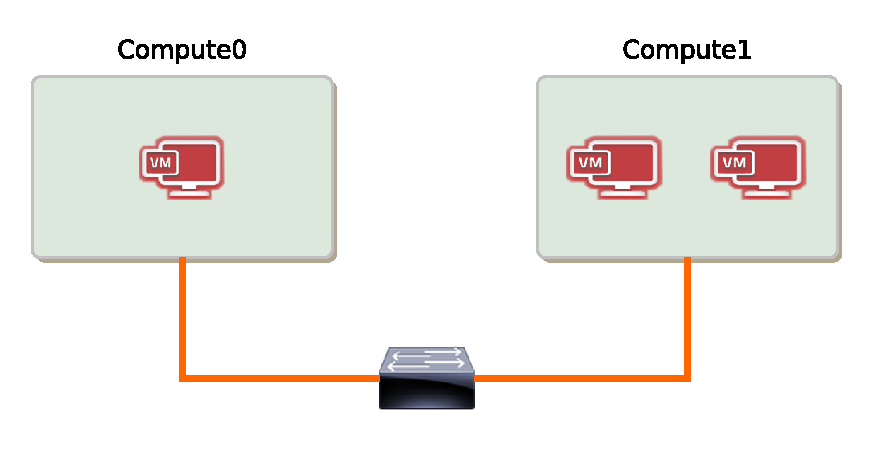
\includegraphics[width=0.8\textwidth]{diagrama.pdf}
    \caption{Esta es una figura que latex decide donde colocar (floating) en el documento.}
    \label{fig:diagrama}
    \end{figure}

  \begin{tabular}{cc}
    Imagen 1 & Imagen 2 \\[2mm]
    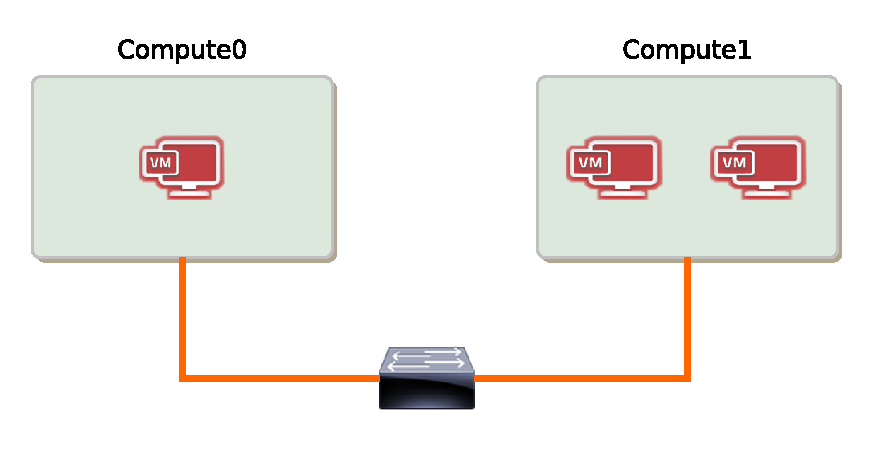
\includegraphics[width=0.4\textwidth]{diagrama.pdf} &  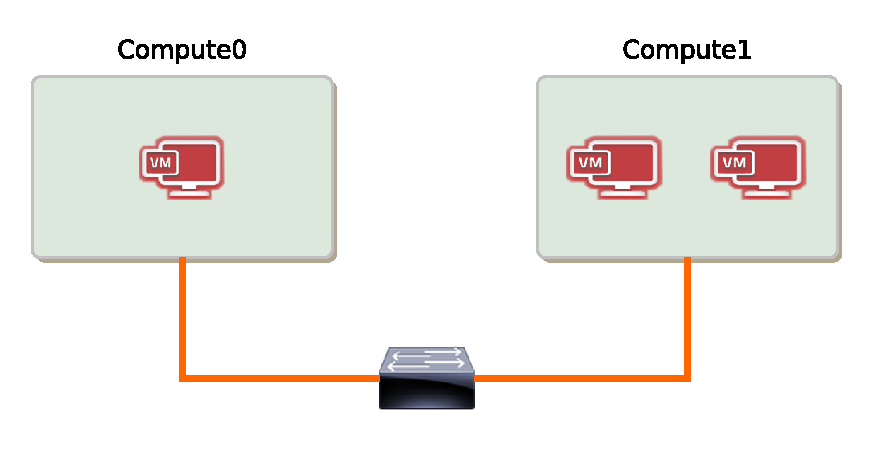
\includegraphics[width=0.4\textwidth]{diagrama.pdf}
  \end{tabular}
  
  Este es un ejemplo de una tabla:
  
  \begin{tabular}{|l|c|}
    \hline
    Columna 1 & Columna 2 \\ \hline
    1 & 2 \\ \hline
  \end{tabular}


  \vspace*{1cm}
  O la misma tabla centrada:

  \begin{center}
    \begin{tabular}{|l|c|}
      \hline
      Columna 1 & Columna 2 \\ \hline
      1 & 2 \\ \hline
    \end{tabular}
  \end{center}

  Para generar el fichero PDF:
  
  \begin{lstlisting}{language=bash}
    pdflatex ejemplo-memoria.tex
    bibtex ejemplo-memoria
    pdflatex ejemplo-memoria.tex
\end{lstlisting}

  También se puede usar \texttt{latexmk} que automáticamente regenera la bibliografía.
  \begin{lstlisting}{language=bash}
    latexmk -pdf ejemplo-memoria.tex
\end{lstlisting}

  
	
	\addcontentsline{toc}{chapter}{Bibliografía}
	\bibliographystyle{unsrt}
	\bibliography{bib/bibliografia}
	
	
	
	
\end{document}

%%% Local Variables:
%%% mode: latex
%%% TeX-master: t
%%% End:
